\documentclass[12pt,a4paper]{article}
\usepackage{graphicx}
\usepackage{gensymb}
\usepackage{amsmath}
\usepackage{bm}
\usepackage{tikz}
\usepackage{float}

\tikzset{
    node distance=2cm, % specifies the minimum distance between two nodes. Change if necessary.
    }
\title{Base Study Modelling an Electronic Component}
\author{
  Azure Hutchings
  \and
  Jean-Luc Danoy
  \and
  Faris Saad S Alsubaie
}
\date{28 October 2019}
 
\begin{document}
 
\begin{titlepage}
\maketitle
\end{titlepage}

\renewcommand{\abstractname}{Executive Summary}
\begin{abstract}
Write Abstract Here
\end{abstract}

\pagebreak

\tableofcontents

\pagebreak

\section{Introduction}

\subsection{Purpose of the Report}
The following report investigates the steady-state heat distribution in a newly designed component. 

The report will discuss the mathematical model of the heat distribution in the component and the numerical methods used to solve it in MATLAB, along with different ways to store the data.

\subsection{The Maths of the Problem}
The component schematic is shown in Appenix A. The location of the component within the device means it's subject to different temperature condition along it's boundaries. The boundary A-B is in perfect thermal contact with another component which the temperature is known to 70\degree C. The boundary C-D is also in perfect thermal contact with another component which the temperature is known to be 40\degree C. The boundary A-E-D is thermally insulated and the boundary B-C is exposed to the air at ambient temperature.
\\\\
This type of model can be described with Laplace's equation. Letting $T(x,y)$ represent the temperature of the component at point $(x, y)$, the model is as follows	

\begin{center}
\begin{tabular}{c c}
$\frac{\partial^2 T}{\partial x^2}+\frac{\partial^2 T}{\partial y^2}=0$ & in the interior\\
$T = 70$ & on boundary A-B \\
$T = 40$ & on boundary C-D \\
$\boldsymbol{\nabla} T \cdot {\hat{\textbf{n}}} = 0$ & on boundary A-E-D\\
$k\boldsymbol{\nabla}T\cdot\hat{\textbf{n}} = h(T_{\infty} - T)$ & on boundary B-C
\end{tabular}
\end{center}
Where the thermal conductivity is $k=3Wm^{-1}C^{-1}$, and the heat transfer coefficient is $h=20 Wm^{-2}C^{-1}$. To begin with, we will assume the ambient termperature is $T_\infty = 20$.
\subsection{Continuous to Discrete}
\clearpage

\section{Finite Difference Mesh}
To discretise the problem, w first construct a mesh of nodes. The problem can then be solved on those individual points to approximate an analytical solution. Given the shape of our component, if we split it into nodes that are 0.01 units away from each other, we can get a mesh that fits nicely along the boundary. This will give us an accurate numerical answer while not being computationally intensive. 
\\
To use this discretisation, we can label each node with it's coordinate $(x,y)$ where x is the row position and y is the column position starting at the bottom left with $(0,0)$. We can use this mesh to create a system of equations for the rate of change of temperature at each point based on the model.
\subsection{The inside of the mesh}
At any point where the node is entirely surrounded by other numbered nodes, we can use the following equation to describe the change of temperature.
\begin{center}
$\frac{\partial u}{\partial t}=D\big{(}\frac{\partial^2 u}{\partial x^2}+\frac{\partial^2 u}{\partial y^2}\big{)}$
\end{center}
As discussed earlier, we can replace the double partial derivative of u with respect to x and y with a second order central difference. %DISCUSS THIS IN THE MATHS OF THE PROBLEM
\begin{center}
$ $
\end{center}


\clearpage
\section{Appendix}
\section*{A}
\begin{figure}[h!]
	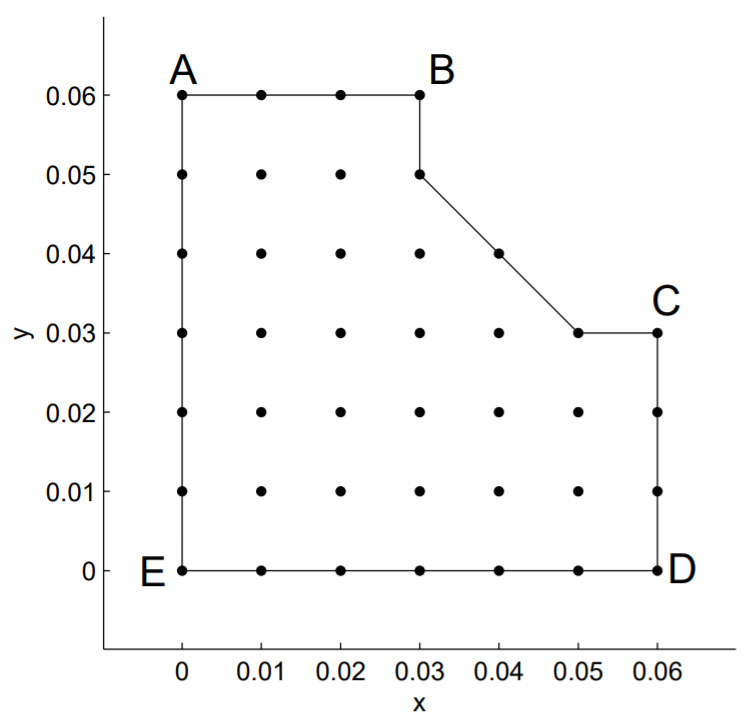
\includegraphics[width=\linewidth]{images/Component.png}
	\caption{Schematic of electronic component.}
	\label{fig:componentSchematic2}
\end{figure}

\section*{B}
\begin{figure}[h!]
	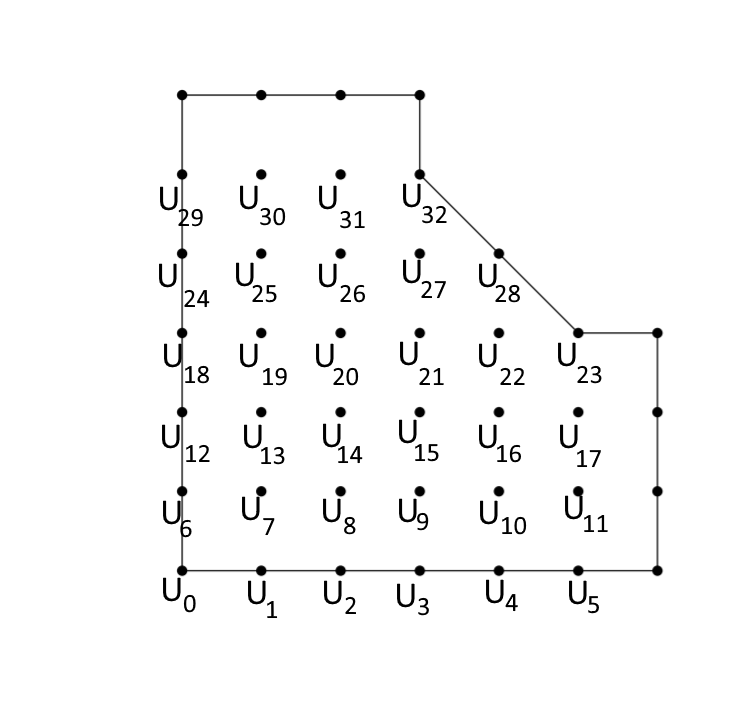
\includegraphics[width=\linewidth]{images/ComponentNodesOrdering.png}
	\caption{Node ordering}
	\label{fig:componentNodes}
\end{figure}

\section*{C}
\begin{center}
$function a=packed_storage(A)
[~,n]=size(A);
a=zeros(1,nchoosek(n+1,2));
for j=1:n
    for i=1:j
       a(i+j*(j-1)/2) = A(i,j);
    end
end$
\end{center}

\end{document}
